
\documentclass[%
  aspectratio=169,
  9pt,
  USenglish,
  titlegraphic, % store custom image to .images/titlegraphic
  %affiliationintitlepagehead,
  progressbar,
%   affiliation,
]{beamer}
%\texttt{}

\usetheme{TUM}


\newcommand{\coorg}{Irisa}


\setbeamertemplate{blocks}[rounded][shadow=false]

\usepackage{tikz}  
\usepackage{tikz-3dplot} 
\usepackage{graphicx}
\usepackage{media9}
\usetikzlibrary{positioning}

\usepackage{amsmath}
\usepackage{booktabs}

% change the camera position
\tdplotsetmaincoords{45}{135}

\usepackage{tabularx}

\usepackage{subcaption}

\usepackage{animate}

\usepackage{pgfmath}
\newcommand\randmin{}
\newcommand\randmax{}
\newcommand\randmultof{}
\newcommand\setrand[4]%
{\def\randmin{#1}%
	\def\randmax{#2}%
	\def\randmultof{#3}%
	\pgfmathsetseed{#4}%
}
\newcommand\nextrand
{\pgfmathparse{int(int((rnd*(\randmax-\randmin+1)+\randmin)/\randmultof)*\randmultof)}%
	\xdef\thisrand{\pgfmathresult}%
}

%\usepackage[backend=biber]{biblatex}
%\addbibresource{bib/references.bib}

\newcommand{\wave}{
	\begin{tikzpicture}[xscale=.05,yscale=.2]
	\draw[-,fill=white] plot[domain=0:10*pi,smooth] (\x,{sin(\x r)});
	\end{tikzpicture}
}


\newcommand{\domain}[4]{
	%% spatial,spectral,temporal
	\draw[fill=#4, opacity=.2] (#1,0,0) -- (0,#2,0) -- (0,0,#3) -- (#1,0,0);
}


\newcommand{\radarwave}{
	\begin{tikzpicture}[xscale=.1,yscale=.2]
	\draw[-,fill=white] plot[domain=0:5*pi,smooth] (\x,{sin(\x r)});
	\end{tikzpicture}
}


\newcommand{\earth}{
	\begin{tikzpicture}[baseline=-.25em, inner sep=0]
	\node{\includegraphics[width=8mm]{images/icons/earth}};
	\end{tikzpicture}
}

\newcommand{\sat}{
	\begin{tikzpicture}[baseline=-.25em, inner sep=0]
	\node[rotate=270,anchor=center]{\includegraphics[width=8mm]{images/icons/sat2}};
	\end{tikzpicture}
}


\usepackage[capitalize]{cleveref}
\usepackage[square,sort,comma,numbers]{natbib}

%% this hack seems to be nececessary due to incompatibilities of cvpr template and tikz... -> https://tex.stackexchange.com/questions/398223/tikz-gives-error-command-everyshipouthook-already-defined
%\makeatletter
%\@namedef{ver@everyshi.sty}{}
%\makeatother
%% hackend

\usepackage{tikz}
\usepackage{pgfplots}
\usetikzlibrary{positioning, calc,arrows,arrows.meta, fit}
%\usetikzlibrary{arrows.meta,calc,decorations.markings,math,arrows.meta}
\usepgfplotslibrary{groupplots}
\usepgfplotslibrary{fillbetween}
\usepgfplotslibrary{statistics} % provides boxplots
\usepackage{xfrac}

\newcommand{\tp}{tp}
\newcommand{\tn}{tn}
\newcommand{\fp}{fp}
\newcommand{\fn}{fn}


\usepackage{tumcolors}
\usepackage{tummath}
\newcommand{\yhat}{\hat{\V{y}}}
\newcommand{\ycorrect}{\hat{y}^+}
\newcommand{\thetadelta}{\V{\Theta}_\delta}
\newcommand{\biasdelta}{b_\delta}
\newcommand{\biasclass}{\V{b}_\text{c}}
\newcommand{\thetaclass}{\V{\Theta}_\text{c}}
\newcommand{\thetafeat}{\V{\Theta}_\text{feat}}
\newcommand{\fclass}{f_\text{c}}
\newcommand{\fdelta}{f_\delta}
\newcommand{\ffeat}{f_\text{feat}}
\newcommand{\f}{f}

\newcommand{\rvtime}{T_c} 
\newcommand{\xuptot}{\M{X}_{\rightarrow t}} 
\newcommand{\deltauptot}{\delta_{\rightarrow t}} 
\newcommand{\tstop}{\ensuremath{t_\text{stop}}}
\newcommand{\meantstop}{\ensuremath{\bar{t}_\text{stop}}}
\usepackage[super]{nth}
\usepackage{mathtools}

\definecolor{evalcolor}{HTML}{3F3F3F}
\definecolor{traincolor}{HTML}{B98951}
\definecolor{validcolor}{HTML}{3F4BBE}

\definecolor{fdlcolor}{HTML}{142737}

\usepackage{multimedia}

\colorlet{colortrain}{tumblue}
\colorlet{colorinfer}{tumblack}

\colorlet{earlinesscolor}{tumblue}
\colorlet{accuracycolor}{tumorange}

\colorlet{stdcolor}{tumbluelight}
\colorlet{mediancolor}{tumorange}
\colorlet{meancolor}{tumblue}

\colorlet{b1color}{tumdiagramaubergine}
\colorlet{b2color}{tumdiagramnavyblue}
\colorlet{b3color}{tumdiagramturquoise}
\colorlet{b4color}{tumdiagramgreen}
\colorlet{b5color}{tumdiagramlimegreen}
\colorlet{b6color}{tumdiagramyellow}
\colorlet{b7color}{tumdiagramsand}
\colorlet{b8color}{tumdiagramredorange}
\colorlet{b8Acolor}{tumdiagramred}
\colorlet{b9color}{tumblack}
\colorlet{b10color}{tumblue}
\colorlet{b11color}{tumdiagramdarkred}
\colorlet{b12color}{tumorange}

% atmospheric bands
\colorlet{b1color}{tumblack}%tumdiagramaubergine
\colorlet{b9color}{tumblack}%tumblack
\colorlet{b10color}{tumblack}%tumblue

%visisble bands
\colorlet{b2color}{tumblue}%tumdiagramnavyblue
\colorlet{b3color}{tumblue}%tumdiagramturquoise
\colorlet{b4color}{tumblue}%tumdiagramgreen

% near infrared bands
\colorlet{b5color}{tumdiagramred}%tumdiagramlimegreen
\colorlet{b6color}{tumdiagramred}%tumdiagramyellow
\colorlet{b7color}{tumdiagramred}%tumdiagramsand
\colorlet{b8color}{tumdiagramred}%tumdiagramredorange
\colorlet{b8Acolor}{tumdiagramred}%tumdiagramred

% SWIR bands
\colorlet{b11color}{tumorange}%tumdiagramdarkred
\colorlet{b12color}{tumorange}%tumorange

\colorlet{epsilon0color}{tumorange}
\colorlet{epsilon1color}{tumblue}
\colorlet{epsilon10color}{tumblack}

\colorlet{gridcolor}{tumblue}
\colorlet{activationcolor}{tumorange}

\colorlet{meadowcolor}{tumbluemedium}
\colorlet{wbarleycolor}{tumbluedark}
\colorlet{corncolor}{tumorange}
\colorlet{wheatcolor}{tumgreen}
\colorlet{sbarleycolor}{tumdiagramred}
\colorlet{clovercolor}{tumdiagramturquoise}
\colorlet{triticalecolor}{tumdiagramsand}

\tikzstyle{rnn}=[draw,circle, inner sep=.1em]
\tikzstyle{norm}=[rounded corners,draw]
\tikzstyle{annot}=[rounded corners, fill=tumblue!20]
\tikzstyle{infer}=[-stealth, shorten >=.0em, shorten <=.0em, colorinfer]
\tikzstyle{loss}=[fill=tumblue!10, rounded corners, font=\small]
\tikzstyle{grad}=[colortrain]

\newcommand{\ptoffset}{\varepsilon}

\tikzstyle{test} = [thick]
\tikzstyle{train} = [thin, dotted]

\usepackage[inline]{enumitem}
\setenumerate{label=(\roman*),itemsep=3pt,topsep=3pt}

\setlength{\belowcaptionskip}{-10pt}


\colorlet{traincolor}{tumbluelight}
\colorlet{validcolor}{tumbluedark}
\colorlet{evalcolor}{tumorange}

\colorlet{forwardcolor}{tumblue}
\colorlet{backwardcolor}{tumorange}

% defaultvalue -> might be replaced later
\colorlet{tensorcolor}{forwardcolor}

\colorlet{classcolor}{tumivory}
\colorlet{encodercolor}{tumblue}
\colorlet{encodercolor}{tumblue}
\colorlet{colorblue}{tumblue}
\colorlet{colororange}{tumorange}

\colorlet{colorclassone}{tumblue}
\colorlet{colorclasstwo}{tumblack}
\colorlet{colorclassthree}{tumorange}
\colorlet{colorclassfour}{tumgray}

\colorlet{frh01color}{tumgray}
\colorlet{frh02color}{tumorange}
\colorlet{frh03color}{tumblue}
\colorlet{frh04color}{tumblack}



%\usepackage{media9}

% notation
\newcommand{\MWeight}{\ensuremath{\M{W}}}
\newcommand{\VBias}{\ensuremath{\V{b}}}
\newcommand{\VInput}{\DataVec}
\newcommand{\VHidden}{\ensuremath{\V{h}}}
\newcommand{\FActivation}{\ensuremath{\sigma}}
\newcommand{\VCellState}{\ensuremath{\V{c}}}
\newcommand{\VForgetGate}{\ensuremath{\V{f}}}
\newcommand{\VModulationGate}{\ensuremath{\V{j}}}
\newcommand{\VInputGate}{\ensuremath{\V{i}}}
\newcommand{\VOutputGate}{\ensuremath{\V{o}}}
\newcommand{\concat}[2]{\left[#1 \parallel #2\right]}


\newcommand{\VResetGate}{\ensuremath{\V{r}}}
\newcommand{\VUpdateGate}{\ensuremath{\V{u}}}


%\usepackage{titlesec}
%\titlespacing{\section}{0pt}{10pt}{3pt}


\usetikzlibrary{3d}
\tikzstyle{perspective3d}=[
x={(0.5cm,0.5cm)}, y={(1cm,0cm)}, z={(0cm,1cm)}]


\usetikzlibrary{spy}

\usetikzlibrary{external,pgfplots.dateplot}

\usepackage[eulergreek]{sansmath}
\pgfplotsset{
	y tick label style={/pgf/number format/.cd,%
		scaled y ticks = false,
		set thousands separator={},
		fixed},
	x tick label style={/pgf/number format/.cd,%
		scaled x ticks = false,
		set decimal separator={,},
		fixed},
	tick label style = {font=\scriptsize\sansmath\sffamily},
	every axis label = {
		font=\scriptsize\sansmath\sffamily},
	every axis/.append style={
		axis lines=left, 
		enlargelimits, 
		thick},
	legend style = {font=\scriptsize\sansmath\sffamily, draw=none, rounded corners=0, fill opacity=.5, text opacity=1},
	label style = {font=\scriptsize\sansmath\sffamily},
	grid style={line width=.1pt, draw=gray!10},
	major grid style={line width=.2pt,draw=tumgraylight},
}

%\let\tempone\itemize
%\let\temptwo\enditemize
%\renewenvironment{itemize}{\tempone\addtolength{\itemsep}{-.5\baselineskip}}{\temptwo}

\tikzstyle{circ} = [circle, draw=white, fill=tumblue, inner sep=1pt]
\newcommand{\fcn}{
	\begin{tikzpicture}[scale=0.2, rotate=0, baseline=-.25em, inner sep=1pt]
	\node[circ](a0) at (0,-1){};
	\node[circ](a1) at (0,0){};
	\node[circ](a2) at (0,1){};
	
	\node[circ](b0) at (1,-0.5){};
	\node[circ](b1) at (1,0.5){};
	
	\draw[-] (a0) -- (b0);
	\draw[-] (a1) -- (b0);
	\draw[-] (a2) -- (b0);
	
	\draw[-] (a0) -- (b1);
	\draw[-] (a1) -- (b1);
	\draw[-] (a2) -- (b1);
	
	\end{tikzpicture}
}

\newcommand{\lfcn}[1]{
	\begin{tikzpicture}[scale=#1, rotate=0, baseline=-.25em, inner sep=1pt]
	\node[circle, draw=white, fill=tumblue, inner sep=3](a0) at (0,-1){};
	\node[circle, draw=white, fill=tumblue,  inner sep=3](a1) at (0,0){};
	\node[circle, draw=white, fill=tumblue,  inner sep=3](a2) at (0,1){};
	
	\node[circle, draw=white, fill=tumblue,  inner sep=3](b0) at (1,-0.5){};
	\node[circle, draw=white, fill=tumblue,  inner sep=3](b1) at (1,0.5){};
	
	\draw[-] (a0) -- (b0);
	\draw[-] (a1) -- (b0);
	\draw[-] (a2) -- (b0);
	
	\draw[-] (a0) -- (b1);
	\draw[-] (a1) -- (b1);
	\draw[-] (a2) -- (b1);
	
	\end{tikzpicture}
}

\newcommand{\hidden}[1]{
	\begin{tikzpicture}[scale=.1, baseline=-.25em]	
	%\draw[step=1.0,black,thin] (0,0) grid (#1,1);
	\foreach \i in {1,...,#1}{
		\node[circle, draw=white, fill=tumbluelight, inner sep=1pt] at (\i,0){};
	}
	\end{tikzpicture}
}

\newcommand{\drawvector}[1]{
	\begin{tikzpicture}[scale=.1, baseline=-.25em]	
	%\draw[step=1.0,black,thin] (0,0) grid (#1,1);
	\foreach \i in {1,...,#1}{
		\node[circ] at (\i,0){};
	}
	\end{tikzpicture}
}

\title{Early Classification for Agricultural Monitoring}
\subtitle{from Satellite Time Series}
\author[M. Rußwurm, R. Tavenard, S. Lefèvre, M.Körner]{Marc Rußwurm, Romain Tavenard, Sébastien Lefèvre, Marco Körner}
\institute[TUM, IRISA-Obelix, LETG-Rennes]{Technical University of Munich, Germany\\
                Remote Sensing Technology}
\date{\today}

\begin{document}
\begin{frame}[t]
  \titlepage
\end{frame}



{\setbeamercolor{background canvas}{bg=tumgraylight}
	\begin{frame}[plain]
	\vfill
	\Huge\color{tumbluedark}
	\begin{columns}
		\column{.5\textwidth}
		\vspace{4em}
		
		\hfill \textbf{Early} Time Series \\\hfill Classification
		\column{.5\textwidth}
		
\includegraphics[width=4cm]{images/TUM-blue}
		
		\vspace{1em}
		
\includegraphics[width=7cm]{images/Irisa}
	\end{columns}
	%		
\includegraphics[width=5cm]{images/TUM-white}
	%		
\includegraphics[width=7cm]{images/Irisa}
	
	\vfill
\end{frame}
}


\begin{frame}
\frametitle{Winter Research Stay at IRISA Obelix Lab in France}

\begin{columns}
\column{.5\textwidth}

Research Stay
\begin{itemize}[itemsep=1em]
	\item Prof. \textbf{Sebastien Lefèvre} and Prof. \textbf{Romain Tavenard}
	\item Obelix: \textbf{Environment observation} with \textbf{complex imagery}
	\item Vannes and Rennes, Britanny, France
\end{itemize}

\vspace{1em}
\url{http://www-obelix.irisa.fr/}

\column{.5\textwidth}

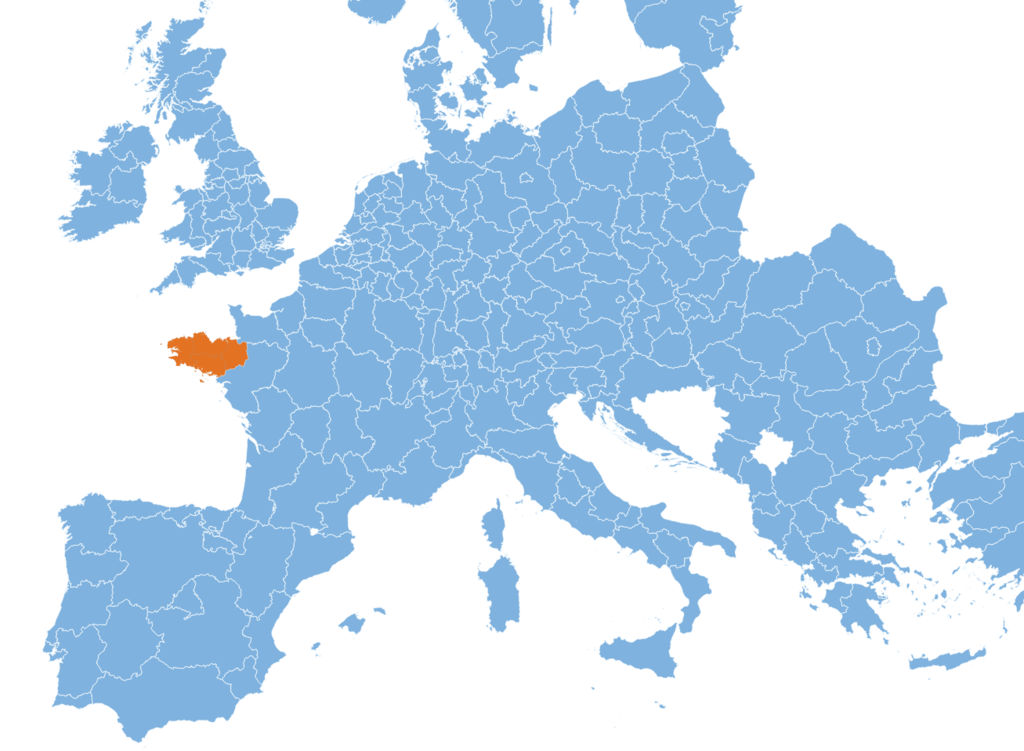
\includegraphics[width=5cm]{images/map/europe}

\end{columns}

\end{frame}


\tikzstyle{rnn}=[draw,circle]
\tikzstyle{annot}=[rounded corners, fill=colorblue!20]
\colorlet{colortrain}{colorblue}
\colorlet{colorinfer}{colororange}
\tikzstyle{infer}=[-stealth, shorten >=.0em, shorten <=.0em, colorinfer]
\tikzstyle{loss}=[fill=colorblue!10, rounded corners, font=\small]
\tikzstyle{grad}=[colortrain]

\newcommand{\classimagepair}[1]{
\def\sample{#1}
\begin{tikzpicture}[node distance=.2em]
\node[label=above:{inputs $\V{x}_t$}](a){\includegraphics[width=.5\textwidth]{images/classification_without_earliness/TwoPatterns30EpochsNoEarliness/sample_\sample_x.png}};
\node[label=above:{softmaxed class scores $\yhat_t$}, right=of a](b){\includegraphics[width=.5\textwidth]{images/classification_without_earliness/TwoPatterns30EpochsNoEarliness/sample_\sample_p(y).png}};

\visible<2->{
%\draw (-2,-2) to[grid with coordinates] (8,4);
\node[annot, yshift=3em](wiggle1) at ($ (a)!0.3!(b) $) {event \#1};
\draw (wiggle1) -- (-1.5,0);
\draw (wiggle1) -- (5.5,-1);
}
\visible<3->{
\node[annot, yshift=-5em](wiggle2) at ($ (a)!0.3!(b) $) {event \#2};
\draw (wiggle2) -- (1,0);
\draw (wiggle2) -- (7.5,0);
}

\visible<4->{
\draw[very thick] (8.5,-2) -- (8.5,2); 
\node[annot, yshift=-5em, anchor=east](stop) at (10,-1) {...we could stop here};
%		\draw[shorten >=1em] (stop)++(2,0.5) -- (8,0);
}
\end{tikzpicture}
}

\begin{frame}<presentation:1-4>{Class Predictions}
\classimagepair{0}
\end{frame}

\begin{frame}
\frametitle{ArXiv Paper: End-to-end Learning for Early Classification of Time Series}

\begin{columns}


\column{.5\textwidth}

Rußwurm, M., Lefèvre, S., Courty, N., Emonet, R., Körner, M., \& Tavenard, R. (2019).\textbf{ End-to-end Learning for Early Classification of Time Series}. arXiv preprint arXiv:1901.10681.

\vspace{1em}
https://github.com/rtavenar/early\_rnn

\column{.5\textwidth}

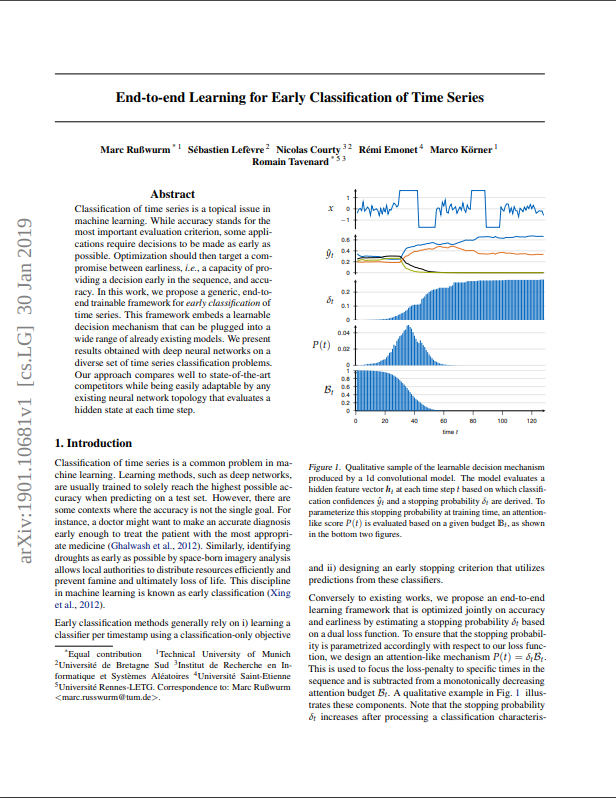
\includegraphics[width=4cm]{images/elects_arxiv}

\end{columns}

\end{frame}



%\begin{frame}
%	\frametitle{Autoregressive Classification Model}
%	
%	\input{images/classmodel.tikz}
%	
%\end{frame}


\begin{frame}
\frametitle{Early Classification on Remote Sensing Data}
\begin{tikzpicture}
	
	\tikzstyle{annot} = [font=\tiny\sffamily, text=tumblue]
	\tikzstyle{point} = [thin, tumbluelight, shorten >= .25em, shorten <= .25em]
	
	% from /home/marc/projects/EV2019/images/example/tstop.txt
	\def\tstopv{0.6285714285714286}
	\def\class{winter barley}
	
	\begin{groupplot}[
	group style={
		group name=my plots,
		group size=1 by 2,
		columns=1,
		xlabels at=edge bottom,
		xticklabels at=edge bottom,
		vertical sep=1em,
	},
	ylabel near ticks,
	ylabel style={font=\sffamily\small, rotate=-90},
	width=\textwidth,
	height=4cm,
	axis x line=bottom,
	axis y line=left,
	enlarge x limits=0.01,
	xtick={0,0.25,0.5,0.75,1},
	xticklabels={January,April,June,Sepember,December},
	ymajorgrids,
	ymin=0, ymax=1.4
	]
	
	\nextgroupplot[thin,
		no marks,  
		ylabel={$\V{x}$},
		draw opacity=.8,
		smooth,
		legend columns=4,
		legend style={at={(.5,1)},anchor=south, line width=1pt, fill=tumblue!10}
		]
		 
	\addplot[b1color] table [x=t, y=B1, col sep=comma, forget plot] {images/example/input.csv};
	\addplot[b9color] table [x=t, y=B9, col sep=comma, forget plot] {images/example/input.csv};
	\addplot[b10color] table [x=t, y=B10, col sep=comma] {images/example/input.csv};
	
	\addplot[b11color] table [x=t, y=B11, col sep=comma, forget plot] {images/example/input.csv};
	\addplot[b12color] table [x=t, y=B12, col sep=comma] {images/example/input.csv};
	
	\addplot[b5color] table [x=t, y=B5, col sep=comma, forget plot] {images/example/input.csv};
	\addplot[b6color] table [x=t, y=B6, col sep=comma, forget plot] {images/example/input.csv};
	\addplot[b7color] table [x=t, y=B7, col sep=comma, forget plot] {images/example/input.csv};
	\addplot[b8color] table [x=t, y=B8, col sep=comma, forget plot] {images/example/input.csv};
	\addplot[b8Acolor] table [x=t, y=B8A, col sep=comma] {images/example/input.csv};
		
	\addplot[b2color] table [x=t, y=B2, col sep=comma, forget plot] {images/example/input.csv};
	\addplot[b3color] table [x=t, y=B3, col sep=comma, forget plot] {images/example/input.csv};
	\addplot[b4color] table [x=t, y=B4, col sep=comma] {images/example/input.csv};
	
	
	\draw[fill=white, draw=none, opacity=.5] (axis cs:\tstopv,0) rectangle (axis cs:1,1.1);
	
	\node[annot](cllab) at (axis cs:.2,1.3) {clouds (noise)};
	\draw[point] (cllab) -- (axis cs:.13,.7);
	\draw[point] (cllab) -- (axis cs:.25,.7);
	\draw[point] (cllab) -- (axis cs:.53,1);
	\draw[point] (cllab) -- (axis cs:.45,.85);
	
	\node[annot](glab) at (axis cs:.8,1.3) {ground (signal)};
	\draw[point] (glab) -- (axis cs:.38,.3);
	\draw[point] (glab) -- (axis cs:.21,.3);
	\draw[point] (glab) -- (axis cs:.7,.3);
	
	\draw (axis cs:\tstopv,0) -- (axis cs:\tstopv,1) node[above]{$\tstop$};
	
	
	
	\legend{3 atmospheric, 2 short-wave infrared, 5 near infrared, 3 visible bands}
	
	\nextgroupplot[thin,
		smooth,
		no marks, 
		ylabel={$\yhat$},
		legend style={at={(.5,-.2)},anchor=north, line width=1pt, fill=tumblue!10},
		legend columns=6]	
	
	\addplot[meadowcolor] table [x=t, y=meadows, col sep=comma] {images/example/proba.csv};
	\addplot[wbarleycolor, thick] table [x=t, y=winter barley, col sep=comma] {images/example/proba.csv};
	\addplot[corncolor] table [x=t, y=corn, col sep=comma] {images/example/proba.csv};
	\addplot[wheatcolor,] table [x=t, y=winter wheat, col sep=comma] {images/example/proba.csv};
	\addplot[sbarleycolor] table [x=t, y=summer barley, col sep=comma] {images/example/proba.csv};
	\addplot[clovercolor] table [x=t, y=clover, col sep=comma] {images/example/proba.csv};
	\addplot[triticalecolor] table [x=t, y=winter triticale, col sep=comma] {images/example/proba.csv};
	
	\draw[fill=white, draw=none, opacity=.5] (axis cs:\tstopv,0) rectangle (axis cs:1,1);
	
	\draw (axis cs:\tstopv,0) -- (axis cs:\tstopv,2.2);
	
	\node[annot](rand) at (axis cs:.1,.8) {first hints};
	\draw[point] (rand) -- (axis cs:.2,.15);
	
	\node[annot](wrong) at (axis cs:.17,1.1) {initially wrong predictions};
	\draw[point] (wrong) -- (axis cs:.25,.7);
	\draw[point] (wrong) -- (axis cs:.4,1);
	
	\node[annot, align=center](corrwait) at (axis cs:.4,1.3) {waiting for more data};
	\draw[point] (corrwait) -- (axis cs:.5,.8);
	
	\node[annot](corr) at (axis cs:.8,1.3) {seen enough data};
	\draw[point] (corr) -- (axis cs:.63,1);
	
	\legend{meadows,\textbf{winter barley},corn,winter wheat,summer barley,clover,winter triticale}
	
	
%	\addplot[thick,colorclassone, name path=y1] table[x=t, y=y1]{\mydata};
%	\addplot[thick,colorclasstwo, name path=y2] table[x=t, y=y2]{\mydata};
%	\addplot[thick,colorclassthree, name path=y3] table[x=t, y=y3]{\mydata};
%	\addplot[thick,colorclassfour, name path=y4] table[x=t, y=y4]{\mydata};
	%\addplot[colorblue!20] fill between[of = y1 and axis];
	%\addplot[colorhgray!20] fill between[of = y2 and axis];
	%\addplot[colorgreen!20] fill between[of = y3 and axis];
	%\addplot[colororange!20] fill between[of = y4 and axis];
	
	
	\end{groupplot}
	
	\end{tikzpicture}

\url{https://arxiv.org/abs/1901.10681}


\end{frame}

\begin{frame}
\frametitle{Stopping times per crop Class}

%\tikzsetnextfilename{classboxplots}

\tikzstyle{druschdatum} = [thin, star,star points=3, star point ratio=0.5, inner sep=.15em, draw=tumwhite, fill=tumblue]

\newcommand{\druschdatum}{
	\begin{tikzpicture}[scale=2, baseline=-.25em, inner sep=0]
	\node[druschdatum, inner sep=.25em]{};
	\end{tikzpicture}
}


\begin{tikzpicture}

\tikzstyle{boxstyle}=[
	mark options={
	draw=tumblue,
	scale=0.5},
	mark=*,
	solid,
	draw=black]

\begin{axis}[
ytick={1,2,3,4,5,6,7},
yticklabels={
	meadows,
	winter barley,
	corn,
	winter wheat,
	summer barley,
	clover,
	winter triticale},
xmajorgrids,
height=6cm,
xmin = 0,
xmax = 1,
ymin = 1,
ymax = 8,
width=\linewidth,
y axis line style={draw=none},
xtick={0,0.1666666667,0.4166666667,0.6666666667,0.9166666667},
xticklabels={January,March,June,September,December},
xlabel={stopping date $\tstop$}
]


%% august <- recommended end of period
% 0.6666666667
\draw [fill=tumbluelight, opacity=.4, draw=none] (axis cs:0.1666666667,0) rectangle (axis cs:0.5833333333,8);
\draw[draw=tumgraydark] (axis cs:0.5833333333,0) -- (axis cs:0.5833333333,8);

\node[font=\tiny\sffamily] at (axis cs:0.37,8.2){vegetative season};

%\node[font=\tiny\sffamily] at (axis cs:0.8,8.2){b};


\addplot+[boxplot, fill=meadowcolor, boxstyle] table[x = meadows, col sep=comma]{images/logs/data/early_reward_p2/classes/meadows.csv};
%
%\addplot+[fill=meadowcolor, draw=black,
%boxplot prepared={
%median=0.4857142857142857,
%upper quartile=0.4,
%lower quartile=0.5857142857142857,
%upper whisker=0.8642857142857143,
%lower whisker=0.12142857142857144,
%} ] coordinates {};

\addplot+[boxplot, fill=wbarleycolor, boxstyle] table[x=winter barley, col sep=comma]{images/logs/data/early_reward_p2/classes/winter_barley.csv};


%
%\addplot+[fill=wbarleycolor, draw=black,
%boxplot prepared={
%median=0.42857142857142855,
%upper quartile=0.37142857142857144,
%lower quartile=0.5857142857142857,
%upper whisker=0.9071428571428573,
%lower whisker=0.04999999999999999,
%} ] coordinates {};


\addplot+[boxplot, fill=corncolor, boxstyle] table[x =corn, col sep=comma]{images/logs/data/early_reward_p2/classes/corn.csv};
%
%\addplot+[fill=corncolor, draw=black,
%boxplot prepared={
%median=0.45714285714285713,
%upper quartile=0.42857142857142855,
%lower quartile=0.5142857142857142,
%upper whisker=0.6428571428571428,
%lower whisker=0.30000000000000004,
%} ] coordinates {};

\addplot+[boxplot, fill=wheatcolor, boxstyle] table[x =winter wheat, col sep=comma]{images/logs/data/early_reward_p2/classes/winter_wheat.csv};


%
%\addplot+[fill=wheatcolor, draw=black,
%boxplot prepared={
%median=0.5285714285714286,
%upper quartile=0.45714285714285713,
%lower quartile=0.5857142857142857,
%upper whisker=0.7785714285714287,
%lower whisker=0.26428571428571423,
%} ] coordinates {};

\addplot+[boxplot, fill=sbarleycolor, boxstyle] table[x =summer barley, col sep=comma]{images/logs/data/early_reward_p2/classes/summer_barley.csv};

%\addplot+[fill=sbarleycolor, draw=black,
%boxplot prepared={
%median=0.37142857142857144,
%upper quartile=0.2857142857142857,
%lower quartile=0.5428571428571428,
%upper whisker=0.9285714285714285,
%lower whisker=-0.09999999999999998,
%} ] coordinates {};

\addplot+[boxplot, fill=clovercolor, boxstyle] table[x=clover, col sep=comma]{images/logs/data/early_reward_p2/classes/clover.csv};

%\addplot+[fill=clovercolor, draw=black,solid,
%boxplot prepared={
%median=0.5,
%upper quartile=0.42857142857142855,
%lower quartile=0.6142857142857143,
%upper whisker=0.892857142857143,
%lower whisker=0.14999999999999986,
%} ] coordinates {};

\addplot+[boxplot, fill=triticalecolor, boxstyle] table[x=winter triticale, col sep=comma]{images/logs/data/early_reward_p2/classes/winter_triticale.csv};

\def\triticale{0.5722222222}
\def\sbarley{0.5833333333}
\def\wbarley{0.5388888889}
\def\wheat{0.5694444444}


% triticale drusch datum 26.07.
%\draw (axis cs:0.524537037,6.5) -- (axis cs:0.524537037,7.5);
\node[druschdatum] at (axis cs:\triticale,7){};

%  summer barley drusch datum 1.8.
%\draw (axis cs:\sbarley,4.5) -- (axis cs:\sbarley,5.5);
\node[druschdatum] at (axis cs:\sbarley,5){};


% winter wheat drusch datum 26.07.
%\draw (axis cs:\wheat,3.5) -- (axis cs:\wheat,4.5);
\node[druschdatum] at (axis cs:\wheat,4){};


% winter barley datum 15.07.
%\draw (axis cs:\wbarley,1.5) -- (axis cs:\wbarley,2.5);
\node[druschdatum] at (axis cs:\wbarley,2){};


%\addplot+[fill=triticalecolor, draw=black,solid,
%boxplot prepared={
%median=0.5571428571428572,
%upper quartile=0.5142857142857142,
%lower quartile=0.6142857142857143,
%upper whisker=0.7642857142857145,
%lower whisker=0.3642857142857141,
%} ] coordinates {};

\end{axis}
\end{tikzpicture} 

\end{frame}

\begin{frame}
\frametitle{Impact of Early Classification on Vegetation Data}

\Large

\begin{itemize}[itemsep=1em]
\item<1-> \textbf{supervised end-to-end} learning scenario
\item<2-> we get a stopping time \textbf{for free} solely from classifying labels
\item<3-> relate to \textbf{characteristic features}, i.e., \textbf{crop phenology}
\item<4-> next: assess seasonal shifts in \textbf{vegetation phenology} due to \textbf{environmental conditions}
\end{itemize}

\end{frame}

\begin{frame}
	\frame{AOI}
	
	\begin{columns}
		\column{.5\textwidth}
			\centering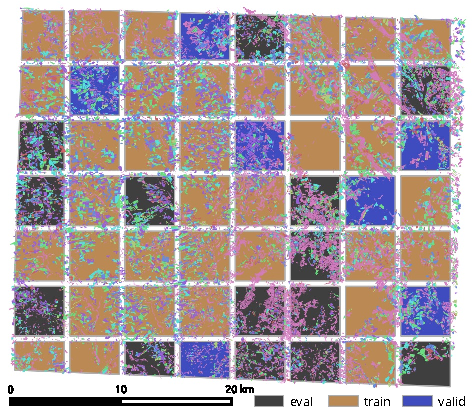
\includegraphics[width=3cm]{images/holl.pdf}
			The area of interest and partitioning in blocks of 4.5 km for training validation and evaluation
			
		\column{.5\textwidth}
			\tikzsetnextfilename{partition_histograms}
\begin{tikzpicture}
  \centering
  \begin{axis}[
        ybar, axis on top,
        title={},
        height=6cm, width=\textwidth,
        bar width=0.2cm,
        ymajorgrids, tick align=inside,
        major grid style={draw=tumgraylight},
        enlarge y limits={value=.1,upper},
        ymin=0, ymax=60,
        axis x line*=bottom,
        axis y line*=left,
        %ymode=log,
        y axis line style={opacity=0},
        tickwidth=0pt,
        enlarge x limits=true,
        legend style={
            at={(1,0.85)},
            anchor=north east,
            draw=none,
            legend columns=-1,
            rounded corners=0,
            /tikz/every even column/.append style={column sep=0.5cm}
        },
        ylabel={Häufigkeit (\%)},
        symbolic x coords={Wiesen,Sommergerste,Silomais,Winterweizen,Wintergerste,Kleegras,Wintertritikale},
       xtick=data,
       tick label style={rotate=0},
       tick label style={rotate=45,anchor=east},
       ylabel near ticks,
       %nodes near coords={
       % \tiny \pgfmathprintnumber[precision=0]{\pgfplotspointmeta}
       %}
    ]
    \addplot [draw=none, fill=traincolor] coordinates {
(Wiesen, 49.506024096385545)
(Sommergerste, 13.560240963855422)
(Silomais, 9.632530120481928)
(Winterweizen, 8.072289156626505)
(Wintergerste, 8.05421686746988)
(Kleegras, 7.530120481927711)
(Wintertritikale, 3.644578313253012)
  };
   \addplot [draw=none,fill=validcolor] coordinates {
(Wiesen, 49.88550866862938)
(Sommergerste, 13.706247955511941)
(Silomais, 9.846254497873733)
(Winterweizen, 8.897612037945699)
(Wintergerste, 8.27608766764802)
(Kleegras, 6.182531894013739)
(Wintertritikale, 3.205757278377494)
  };
   \addplot [draw=none, fill=evalcolor] coordinates {
(Wiesen, 57.32753103801357)
(Sommergerste, 11.852041469345961)
(Silomais, 8.524254447715347)
(Winterweizen, 6.962754383719442)
(Wintergerste, 6.220401894278766)
(Kleegras, 4.876487904774095)
(Wintertritikale, 4.236528862152822)
  };

    \legend{train,valid,eval}
  \end{axis}
  \end{tikzpicture}
			{Class distribution in the dataset with block-wise separation of train, valid and evaluation partitions.}
	
\end{columns}
\end{frame}

\begin{frame}
	
	
	\newcommand{\figearlyreward}{
\def\datapath{images/logs/data/early_reward_p2/classes}
\tikzsetnextfilename{loss-accuracyplots}
\begin{tikzpicture}
	\begin{groupplot}[
	group style = {
		group size = 1 by 2,
		x descriptions at=edge bottom,
		vertical sep=1em},
	no markers,
	height=4cm,
%	legend style={at={(0.03,0.5)},anchor=west},
	width=\linewidth,
	xlabel=epochs
 	]
	\nextgroupplot[legend columns=3, ylabel=loss]

	\addplot[test, tumblack] table [x=epoch, y=loss, col sep=comma] {\datapath/log_earliness_test.csv};
	
	\addplot[test, accuracycolor] table [x=epoch, y=loss_classification, col sep=comma] {\datapath/log_earliness_test.csv};
	
	\addplot[test, earlinesscolor] table [x=epoch, y=earliness_reward, col sep=comma] {\datapath/log_earliness_test.csv};
	
%	\legend{total loss (eval), classification loss (eval), earliness reward (eval)}
%	
	\legend{$(\mathcal{L}_\text{c} - \mathcal{R}_\text{e})$, $\mathcal{L}_\text{c}$, $\mathcal{R}_\text{e}$}
	
	
	
	\nextgroupplot[
		legend columns=2, 
		legend pos=south east,
		ytick={0,0.5,1},
		yticklabels={
			0 ({\color{earlinesscolor} jan}),
			0.5 ({\color{earlinesscolor} jun}),
			1 ({\color{earlinesscolor} dec})},
		ylabel=accuracy/$\meantstop$]
	\addplot[test, accuracycolor] table [x=epoch, y=accuracy, col sep=comma] {\datapath/log_earliness_test.csv};
	\addplot[test, earlinesscolor] table [x=epoch, y=earliness, col sep=comma] {\datapath/log_earliness_test.csv};

	\legend{accuracy,$\meantstop$}
	
	\end{groupplot}
\end{tikzpicture}

}

\newcommand{\figtwophasecrossentropy}{
\begin{tikzpicture}
\begin{groupplot}[
group style = {
	group size = 1 by 2,
	x descriptions at=edge bottom,
	vertical sep=1em},
no markers,
height=2.8cm,
%	legend style={at={(0.03,0.5)},anchor=west},
width=\linewidth,
ymin=0,ymax=2.5,
xlabel=epochs
]
\nextgroupplot[legend columns=3, ylabel=loss,
legend style={at={(1,.85)}, anchor=north east}]

\addplot[test, tumblack] table [x=epoch, y=loss, col sep=comma] {images/logs/data/twophasecrossentropy/log_earliness_test.csv};

\addplot[test, accuracycolor] table [x=epoch, y=loss_classification, col sep=comma] {images/logs/data/twophasecrossentropy/log_earliness_test.csv};

\addplot[test, earlinesscolor] table [x=epoch, y=loss_earliness, col sep=comma] {images/logs/data/twophasecrossentropy/log_earliness_test.csv};

\draw[draw, thick] (axis cs:50,0) -- (axis cs:50,2) node[above, font=\sffamily\scriptsize](s){switch epoch};
\node[left=1em of s, font=\sffamily\scriptsize]{accuracy only};
\node[right=1em of s, font=\sffamily\scriptsize]{accuracy+earliness};

\legend{$(\mathcal{L}_\text{c} + \mathcal{L}_\text{e})$, $\mathcal{L}_\text{c}$, $\mathcal{L}_\text{e}$}

\nextgroupplot[
legend columns=2, 
ytick={0,0.5,1},
ymin=0,ymax=1,
legend style={at={(1,0)}, anchor=south east},
yticklabels={
	0 ({\color{earlinesscolor} jan}),
	0.5 ({\color{earlinesscolor} jun}),
	1 ({\color{earlinesscolor} dec})},
ylabel=accuracy/$\meantstop$]
\addplot[test, accuracycolor] table [x=epoch, y=accuracy, col sep=comma] {images/logs/data/twophasecrossentropy/log_earliness_test.csv};
\addplot[test, earlinesscolor] table [x=epoch, y=earliness, col sep=comma] {images/logs/data/twophasecrossentropy/log_earliness_test.csv};

\legend{accuracy,$\meantstop$}

\draw[draw, thick] (axis cs:50,0) -- (axis cs:50,1.1);

\end{groupplot}
\end{tikzpicture}

}


	\begin{columns}
	\column{.5\textwidth}
\figtwophasecrossentropy
{two-phase training first optimizing for accuracy-only and then for early classifications as well using \emph{lateness penalty} loss.}

	\column{.5\textwidth}
\figearlyreward
{one training phase using the \emph{earliness reward} formulation.}
\end{columns}
	
	
\end{frame}


\begin{frame}

	
	\begin{table}
		\caption{Varying the weighting factor $\alpha$ for the two loss formulations \emph{early reward} (\cref{sec:earlynessreward}) and \emph{lateness penalty} (\cref{sec:twophasecrossentropy}).}
		\label{tab:alpha}
		
		\setlength{\belowcaptionskip}{0pt}
		
		\begin{subtable}{.5\textwidth}
			\scriptsize
			\hspace{0em}\begin{tabular}{lcccccc}
				\toprule
				\textbf{$\alpha$} & accuracy & $\meantstop$ & precision & recall & $f_1$ & $\kappa$ \\
				\cmidrule(lr){0-0}\cmidrule(lr){1-1}\cmidrule(lr){2-2}\cmidrule(lr){3-3}\cmidrule(lr){4-4}\cmidrule(lr){5-5}\cmidrule(lr){6-6}\cmidrule(lr){7-7}
				.0 & .24 $\pm$ .29 & .00 $\pm$ .00 & .04 $\pm$ .04 & .15 $\pm$ .00 & .05 $\pm$ .05 & .00 $\pm$ .00 \\
				.2 & .15 $\pm$ .08 & .00 $\pm$ .00 & .10 $\pm$ .05 & .15 $\pm$ .01 & .08 $\pm$ .03 & .01 $\pm$ .01 \\
				.4 & .79 $\pm$ .05 & .39 $\pm$ .03 & .67 $\pm$ .05 & .71 $\pm$ .04 & .68 $\pm$ .04 & .69 $\pm$ .06 \\
				.6 & .83 $\pm$ .03 & .59 $\pm$ .17 & .71 $\pm$ .03 & .74 $\pm$ .02 & .72 $\pm$ .02 & .74 $\pm$ .04 \\
				.8 & .86 $\pm$ .01 & .86 $\pm$ .12 & .74 $\pm$ .01 & .76 $\pm$ .02 & .75 $\pm$ .02 & .79 $\pm$ .01 \\
				1.0 & .86 $\pm$ .01 & 1.00 $\pm$ .00 & .75 $\pm$ .02 & .76 $\pm$ .02 & .75 $\pm$ .02 & .79 $\pm$ .02 \\
				\bottomrule
			\end{tabular}
			\caption{two-phase \emph{lateness penalty} loss formulation}
			\label{tab:alpha:xentropy}
		\end{subtable}
		\begin{subtable}{.5\textwidth}
			\scriptsize
			\hspace{0em}\begin{tabular}{lcccccc}
				\toprule\small
				\textbf{$\alpha$} & accuracy & $\meantstop$  & precision & recall & $f_1$ & $\kappa$ \\
				\cmidrule(lr){0-0}\cmidrule(lr){1-1}\cmidrule(lr){2-2}\cmidrule(lr){3-3}\cmidrule(lr){4-4}\cmidrule(lr){5-5}\cmidrule(lr){6-6}\cmidrule(lr){7-7}
				.0 & .25 $\pm$ .22 & .10 $\pm$ .17 & .19 $\pm$ .20 & .25 $\pm$ .17 & .16 $\pm$ .20 & .12 $\pm$ .19 \\
				.2 & .81 $\pm$ .03 & .40 $\pm$ .02 & .70 $\pm$ .01 & .74 $\pm$ .01 & .71 $\pm$ .01 & .71 $\pm$ .04 \\
				.4 & .80 $\pm$ .09 & .47 $\pm$ .03 & .71 $\pm$ .02 & .74 $\pm$ .01 & .71 $\pm$ .02 & .71 $\pm$ .10 \\
				.6 & .85 $\pm$ .02 & .88 $\pm$ .07 & .73 $\pm$ .04 & .74 $\pm$ .03 & .73 $\pm$ .03 & .77 $\pm$ .03 \\
				.8 & .84 $\pm$ .01 & .93 $\pm$ .05 & .72 $\pm$ .02 & .75 $\pm$ .01 & .73 $\pm$ .02 & .76 $\pm$ .02 \\
				1.0 & .83 $\pm$ .03 & 1.00 $\pm$ .00 & .72 $\pm$ .03 & .75 $\pm$ .01 & .72 $\pm$ .03 & .75 $\pm$ .04 \\
				\bottomrule
			\end{tabular}
			\caption{one phase \emph{early-reward} formulation}
			\label{tab:alpha:earlyreward}
		\end{subtable}
		
	\end{table}

\end{frame}

\begin{frame}
	
		\newcommand{\figepsilonzero}{
\def\datapath{images/logs/data/epsilon0}
\tikzsetnextfilename{epsilonexperiment}
\begin{tikzpicture}
	\begin{groupplot}[
	group style = {
		group size = 1 by 3,
		x descriptions at=edge bottom,
		vertical sep=.5em},
	no markers,
	height=2.8cm,
%	legend style={at={(0.03,0.5)},anchor=west},
	legend style={at={(1,1)},anchor=south east},
	width=\linewidth,
	xlabel=epochs,
	legend columns=3, 
	ytick={0,0.5,1},
	yticklabels={0,0.5,1},
	ylabel=$\meantstop$
 	]
%	\nextgroupplot[legend columns=1, ylabel=loss]
%
%	\addplot[epsilon10color] table [x=epoch, y=loss_classification, col sep=comma] {images/logs/data/epsilon10/log_earliness_test.csv};
%	\addplot[epsilon10color] table [x=epoch, y=earliness_reward, col sep=comma] {images/logs/data/epsilon10/log_earliness_test.csv};
%	
%	\addplot[epsilon1color] table [x=epoch, y=loss_classification, col sep=comma] {images/logs/data/epsilon1/log_earliness_test.csv};
%	\addplot[epsilon1color] table [x=epoch, y=earliness_reward, col sep=comma] {images/logs/data/epsilon1/log_earliness_test.csv};
%	
%	\addplot[epsilon0color] table [x=epoch, y=loss_classification, col sep=comma] {images/logs/data/epsilon0/log_earliness_test.csv};
%	\addplot[epsilon0color] table [x=epoch, y=earliness_reward, col sep=comma] {images/logs/data/epsilon0/log_earliness_test.csv};
%	
%	
%%	\legend{total loss (eval), classification loss (eval), earliness reward (eval)}
%%	
%	\legend{$\mathcal{L}_\text{c} - \mathcal{R}_\text{e}$, $\mathcal{L}_\text{c}$, $\mathcal{R}_\text{e}$}
%	
	
	
	\nextgroupplot[]
	\legend{$\epsilon = 10$,$\epsilon = 1$,$\epsilon = 0$,}
	
	\addplot[epsilon10color] table [x=epoch, y=earliness, col sep=comma] {images/logs/data/epsilon10_r0/log_earliness_test.csv};
	\addplot[epsilon1color] table [x=epoch, y=earliness, col sep=comma] {images/logs/data/epsilon1_r0/log_earliness_test.csv};
	\addplot[epsilon0color] table [x=epoch, y=earliness, col sep=comma] {images/logs/data/epsilon0_r0/log_earliness_test.csv};
	
	\nextgroupplot[]
	
	\addplot[epsilon10color] table [x=epoch, y=earliness, col sep=comma] {images/logs/data/epsilon10_r1/log_earliness_test.csv};
	\addplot[epsilon1color] table [x=epoch, y=earliness, col sep=comma] {images/logs/data/epsilon1_r1/log_earliness_test.csv};
	\addplot[epsilon0color] table [x=epoch, y=earliness, col sep=comma] {images/logs/data/epsilon0_r1/log_earliness_test.csv};
	
	
	\nextgroupplot[]
	
	\addplot[epsilon10color] table [x=epoch, y=earliness, col sep=comma] {images/logs/data/epsilon10_r2/log_earliness_test.csv};
	\addplot[epsilon1color] table [x=epoch, y=earliness, col sep=comma] {images/logs/data/epsilon1_r2/log_earliness_test.csv};
	\addplot[epsilon0color] table [x=epoch, y=earliness, col sep=comma] {images/logs/data/epsilon0_r2/log_earliness_test.csv};
	
	
	
	
	\end{groupplot}
\end{tikzpicture}

}
		\figepsilonzero
		{The three runs with different random initialization per $\ptoffset$ offset and $\alpha=0.4$ of \cref{tab:epsilon:a04}.
			The $\ptoffset>0$ offset factor allows the models to recover from a too early classification, as is visible in the top two plots.}
	
\end{frame}

\begin{frame}
	
	
	\begin{table}
		\caption{Quantitative analysis of the $\ptoffset$ parameter on different trade-off factors between $\alpha$ earliness and accuracy. The illustrated figures show the mean and standard deviation of three runs with same parameters, but different initial random initialization.}
		\label{tab:epsilon:quantitative}
		\setlength{\belowcaptionskip}{0pt}
		
		\begin{subtable}{.5\textwidth}
			\scriptsize
			%\begin{tabular}{lcccccc}
			%	\toprule
			%	\textbf{$\ptoffset$} & accuracy & earliness & $f_1$ & precision & recall & $\kappa$ \\
			%	\cmidrule(lr){0-0}\cmidrule(lr){1-1}\cmidrule(lr){2-2}\cmidrule(lr){3-3}\cmidrule(lr){4-4}\cmidrule(lr){5-5}\cmidrule(lr){6-6}\cmidrule(lr){7-7}
			%0 & .05 $\pm$ .00 & .00 $\pm$ .00 & .01 $\pm$ .00 & .01 $\pm$ .00 & .14 $\pm$ .00 & .00 $\pm$ .00 \\
			%1 & .41 $\pm$ .26 & .08 $\pm$ .13 & .12 $\pm$ .09 & .11 $\pm$ .09 & .19 $\pm$ .07 & .11 $\pm$ .17 \\
			%10 & .25 $\pm$ .22 & .10 $\pm$ .17 & .16 $\pm$ .20 & .19 $\pm$ .20 & .25 $\pm$ .17 & .12 $\pm$ .19 \\
			%	\bottomrule
			%\end{tabular}
			%\caption{\emph{$\alpha=0$}}
			%\label{tab:epsilon:a0}
			\hspace{-1em}\begin{tabular}{lcccccc}
				\toprule
				\textbf{$\ptoffset$} & accuracy & $\meantstop$  & $f_1$ & precision & recall & $\kappa$ \\
				\cmidrule(lr){0-0}\cmidrule(lr){1-1}\cmidrule(lr){2-2}\cmidrule(lr){3-3}\cmidrule(lr){4-4}\cmidrule(lr){5-5}\cmidrule(lr){6-6}\cmidrule(lr){7-7}
				0 & .10 $\pm$ .02 & .02 $\pm$ .00 & .07 $\pm$ .01 & .13 $\pm$ .06 & .17 $\pm$ .00 & .02 $\pm$ .00 \\
				1 & .75 $\pm$ .09 & .44 $\pm$ .06 & .65 $\pm$ .05 & .64 $\pm$ .03 & .69 $\pm$ .03 & .64 $\pm$ .10 \\
				10 & .81 $\pm$ .03 & .40 $\pm$ .02 & .71 $\pm$ .01 & .70 $\pm$ .01 & .74 $\pm$ .01 & .71 $\pm$ .04 \\
				\bottomrule
			\end{tabular}
			\caption{\emph{$\alpha=0.2$}}
			\label{tab:epsilon:a02}
		\end{subtable}
		\begin{subtable}{.5\textwidth}
			\scriptsize
			\hspace{-1em}\begin{tabular}{lcccccc}
				\toprule
				\textbf{$\ptoffset$} & accuracy & $\meantstop$  & $f_1$ & precision & recall & $\kappa$ \\
				\cmidrule(lr){0-0}\cmidrule(lr){1-1}\cmidrule(lr){2-2}\cmidrule(lr){3-3}\cmidrule(lr){4-4}\cmidrule(lr){5-5}\cmidrule(lr){6-6}\cmidrule(lr){7-7}
				0 & .21 $\pm$ .20 & .02 $\pm$ .00 & .09 $\pm$ .04 & .18 $\pm$ .03 & .16 $\pm$ .01 & .04 $\pm$ .03 \\
				1 & .80 $\pm$ .02 & .50 $\pm$ .05 & .68 $\pm$ .05 & .67 $\pm$ .05 & .70 $\pm$ .07 & .70 $\pm$ .03 \\
				10 & .80 $\pm$ .09 & .47 $\pm$ .03 & .71 $\pm$ .02 & .71 $\pm$ .02 & .74 $\pm$ .01 & .71 $\pm$ .10 \\
				\bottomrule
			\end{tabular}
			\caption{\emph{$\alpha=0.4$}}
			\label{tab:epsilon:a04}
		\end{subtable}
		\begin{subtable}{.5\textwidth}
			\scriptsize
			\hspace{-1em}\begin{tabular}{lcccccc}
				\toprule
				\textbf{$\ptoffset$} & accuracy & $\meantstop$  & $f_1$ & precision & recall & $\kappa$ \\
				\cmidrule(lr){0-0}\cmidrule(lr){1-1}\cmidrule(lr){2-2}\cmidrule(lr){3-3}\cmidrule(lr){4-4}\cmidrule(lr){5-5}\cmidrule(lr){6-6}\cmidrule(lr){7-7}
				0 & .13 $\pm$ .04 & .02 $\pm$ .00 & .08 $\pm$ .01 & .16 $\pm$ .01 & .16 $\pm$ .01 & .02 $\pm$ .01 \\
				1 & .80 $\pm$ .05 & .85 $\pm$ .14 & .71 $\pm$ .02 & .70 $\pm$ .02 & .74 $\pm$ .01 & .70 $\pm$ .06 \\
				10 & .85 $\pm$ .02 & .88 $\pm$ .07 & .73 $\pm$ .03 & .73 $\pm$ .04 & .74 $\pm$ .03 & .77 $\pm$ .03 \\
				\bottomrule
			\end{tabular}
			\caption{\emph{$\alpha=0.6$}}
			\label{tab:epsilon:a06}
		\end{subtable}
		\begin{subtable}{.5\textwidth}
			\scriptsize
			\hspace{-1em}\begin{tabular}{lcccccc}
				\toprule
				\textbf{$\ptoffset$} & accuracy & $\meantstop$  & $f_1$ & precision & recall & $\kappa$ \\
				\cmidrule(lr){0-0}\cmidrule(lr){1-1}\cmidrule(lr){2-2}\cmidrule(lr){3-3}\cmidrule(lr){4-4}\cmidrule(lr){5-5}\cmidrule(lr){6-6}\cmidrule(lr){7-7}
				0 & .11 $\pm$ .03 & .03 $\pm$ .01 & .08 $\pm$ .02 & .15 $\pm$ .02 & .17 $\pm$ .01 & .02 $\pm$ .01 \\
				1 & .84 $\pm$ .03 & .98 $\pm$ .03 & .73 $\pm$ .03 & .72 $\pm$ .04 & .75 $\pm$ .02 & .76 $\pm$ .04 \\
				10 & .84 $\pm$ .01 & .93 $\pm$ .05 & .73 $\pm$ .02 & .72 $\pm$ .02 & .75 $\pm$ .01 & .76 $\pm$ .02 \\
				\bottomrule
			\end{tabular}
			\caption{\emph{$\alpha=0.8$}}
			\label{tab:epsilon:a08}
		\end{subtable}
		%\begin{subtable}{.5\textwidth}
		%	\scriptsize
		%	\hspace{-1em}\begin{tabular}{lcccccc}
		%		\toprule
		%		\textbf{$\ptoffset$} & accuracy & $\meantstop$ & $f_1$ & precision & recall & $\kappa$ \\
		%		\cmidrule(lr){0-0}\cmidrule(lr){1-1}\cmidrule(lr){2-2}\cmidrule(lr){3-3}\cmidrule(lr){4-4}\cmidrule(lr){5-5}\cmidrule(lr){6-6}\cmidrule(lr){7-7}
		%0 & .39 $\pm$ .30 & 1.00 $\pm$ .00 & .14 $\pm$ .15 & .13 $\pm$ .15 & .23 $\pm$ .14 & .12 $\pm$ .21 \\
		%1 & .74 $\pm$ .14 & 1.00 $\pm$ .00 & .51 $\pm$ .36 & .50 $\pm$ .36 & .55 $\pm$ .35 & .49 $\pm$ .42 \\
		%10 & .83 $\pm$ .03 & 1.00 $\pm$ .00 & .72 $\pm$ .03 & .72 $\pm$ .03 & .75 $\pm$ .01 & .75 $\pm$ .04 \\
		%		\bottomrule
		%	\end{tabular}
		%	\caption{\emph{$\alpha=1.0$}}
		%	\label{tab:epsilon:a1}
		%\end{subtable}
		
	\end{table}
	
\end{frame}

\begin{frame}
	
	
		\def\datapath{images/logs/data/early_reward_p2/classes}

\tikzsetnextfilename{trainingstoppingclasses}
\begin{tikzpicture}
	\begin{groupplot}[
	group style = {
		group size = 1 by 7,
		x descriptions at=edge bottom,
		vertical sep=.75em},
	title style={
		font=\sffamily\scriptsize,
		at={(0,1)},
		anchor=north west
	},
	ymajorgrids,
	no markers,
	height=2.7cm,
	legend style={at={(0.5,1)},anchor=south},
	width=\linewidth,
	xlabel=epochs,
	ymax=1.1,
	ymin=0.3,
	ylabel=$\tstop$,
	ytick={0,0.25,0.5,0.75,1},
	yticklabels={Jan,Apr,Jun,Sep,Dec}
	]
	\nextgroupplot[title=meadows, legend columns=3]
	\addplot[meancolor] table [x=epoch, y=meadows, col sep=comma] {\datapath/mean.csv};
	\addplot[mediancolor] table [x=epoch, y=meadows, col sep=comma] {\datapath/median.csv};
	\addplot+[name path=upper, draw=none,forget plot] table [x=epoch, y=meadows, col sep=comma] {\datapath/mean+std.csv};
	\addplot+[name path=lower, draw=none,forget plot] table [x=epoch, y=meadows, col sep=comma] {\datapath/mean-std.csv};
	\addplot[stdcolor] fill between[of=lower and upper];
	
	\legend{mean, median, mean $\mp$ std}
	
	\nextgroupplot[title=winter barley]
	\addplot[meancolor] table [x=epoch, y=winter barley, col sep=comma] {\datapath/mean.csv};
	\addplot[mediancolor] table [x=epoch, y=winter barley, col sep=comma] {\datapath/median.csv};
	\addplot+[name path=upper, draw=none] table [x=epoch, y=winter barley, col sep=comma] {\datapath/mean+std.csv};
	\addplot+[name path=lower, draw=none] table [x=epoch, y=winter barley, col sep=comma] {\datapath/mean-std.csv};
	\addplot[stdcolor] fill between[of=lower and upper];
	\nextgroupplot[title=corn]
%	\addplot table [x=epoch, y=corn, col sep=comma] {images/logs/data/early_reward/classes/mean.csv};
	
	\addplot[meancolor] table [x=epoch, y=corn, col sep=comma] {\datapath/mean.csv};
	\addplot[mediancolor] table [x=epoch, y=corn, col sep=comma] {\datapath/median.csv};
	\addplot+[name path=upper, draw=none] table [x=epoch, y=corn, col sep=comma] {\datapath/mean+std.csv};
	\addplot+[name path=lower, draw=none] table [x=epoch, y=corn, col sep=comma] {\datapath/mean-std.csv};
	\addplot[stdcolor] fill between[of=lower and upper];
	
	\nextgroupplot[title=winter wheat]
%	\addplot table [x=epoch, y=winter wheat, col sep=comma] {images/logs/data/early_reward/classes/mean.csv};
%	
	\addplot[meancolor] table [x=epoch, y=winter wheat, col sep=comma] {\datapath/mean.csv};
	\addplot[mediancolor] table [x=epoch, y=winter wheat, col sep=comma] {\datapath/median.csv};
	\addplot+[name path=upper, draw=none] table [x=epoch, y=winter wheat, col sep=comma] {\datapath/mean+std.csv};
	\addplot+[name path=lower, draw=none] table [x=epoch, y=winter wheat, col sep=comma] {\datapath/mean-std.csv};
	\addplot[stdcolor] fill between[of=lower and upper];
	
	\nextgroupplot[title=summer barley]
%	\addplot table [x=epoch, y=winter barley, col sep=comma] {images/logs/data/early_reward/classes/mean.csv};
	
	\addplot[meancolor] table [x=epoch, y=summer barley, col sep=comma] {\datapath/mean.csv};
	\addplot[mediancolor] table [x=epoch, y=summer barley, col sep=comma] {\datapath/median.csv};
	\addplot+[name path=upper, draw=none] table [x=epoch, y=summer barley, col sep=comma] {\datapath/mean+std.csv};
	\addplot+[name path=lower, draw=none] table [x=epoch, y=summer barley, col sep=comma] {\datapath/mean-std.csv};
	\addplot[stdcolor] fill between[of=lower and upper];
	
	\nextgroupplot[title=clover]
%	\addplot table [x=epoch, y=clover, col sep=comma] {images/logs/data/early_reward/classes/mean.csv};
	
	\addplot[meancolor] table [x=epoch, y=clover, col sep=comma] {\datapath/mean.csv};
	\addplot[mediancolor] table [x=epoch, y=clover, col sep=comma] {\datapath/median.csv};
	\addplot+[name path=upper, draw=none] table [x=epoch, y=clover, col sep=comma] {\datapath/mean+std.csv};
	\addplot+[name path=lower, draw=none] table [x=epoch, y=clover, col sep=comma] {\datapath/mean-std.csv};
	\addplot[stdcolor] fill between[of=lower and upper];
	
	\nextgroupplot[title=winter triticale]
%	\addplot table [x=epoch, y=winter triticale, col sep=comma] {images/logs/data/early_reward/classes/mean.csv};

	\addplot[meancolor] table [x=epoch, y=winter triticale, col sep=comma] {\datapath/mean.csv};
	\addplot[mediancolor] table [x=epoch, y=winter triticale, col sep=comma] {\datapath/median.csv};
	\addplot+[name path=upper, draw=none,forget plot] table [x=epoch, y=winter triticale, col sep=comma] {\datapath/mean+std.csv};
	\addplot+[name path=lower, draw=none,forget plot] table [x=epoch, y=winter triticale, col sep=comma] {\datapath/mean-std.csv};
	\addplot[stdcolor] fill between[of=lower and upper];

	
	\end{groupplot}
	\end{tikzpicture}
		{Class-wise analysis of the estimated stopping time during training in the evaluation set.}
	
\end{frame}

\begin{frame}
	\begin{columns}
	\column{.5\textwidth}
	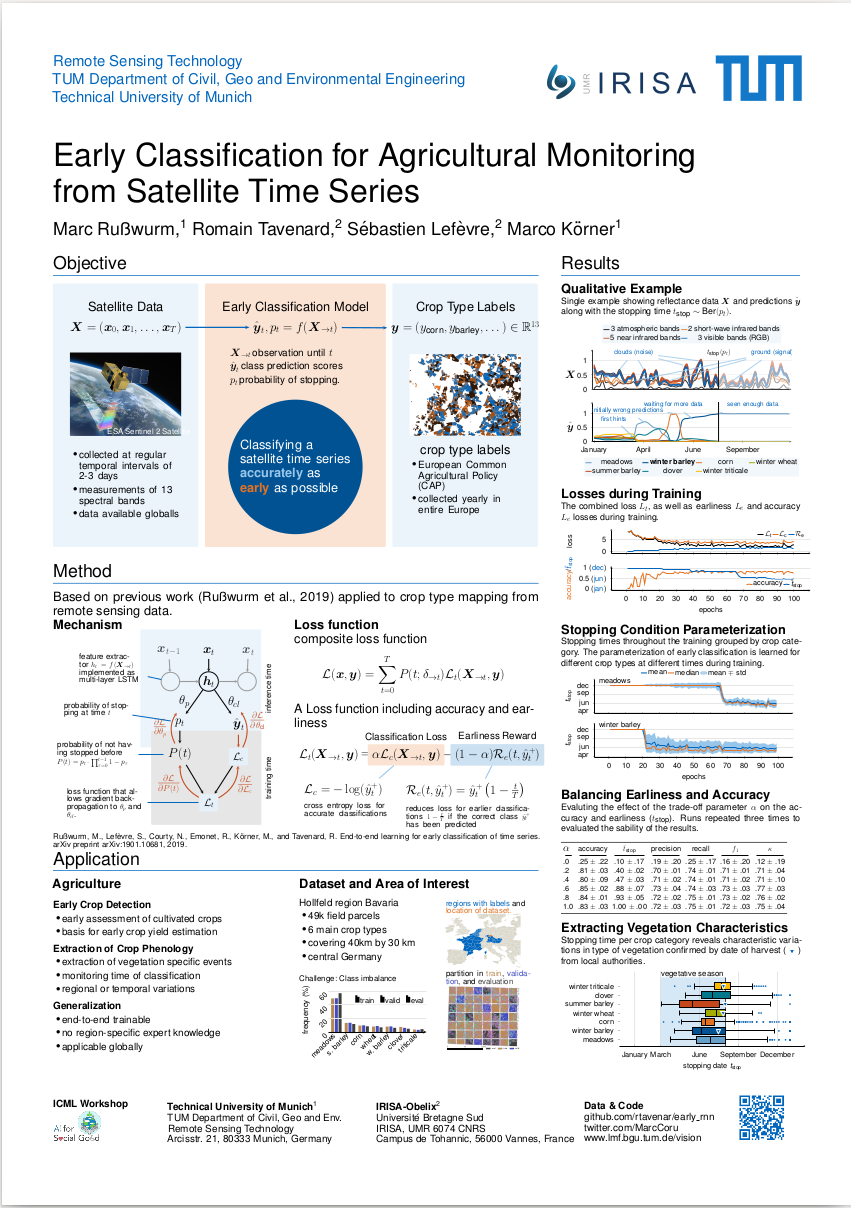
\includegraphics[width=.6\textwidth]{images/AI4SG_Poster}
	
	\column{.5\textwidth}
	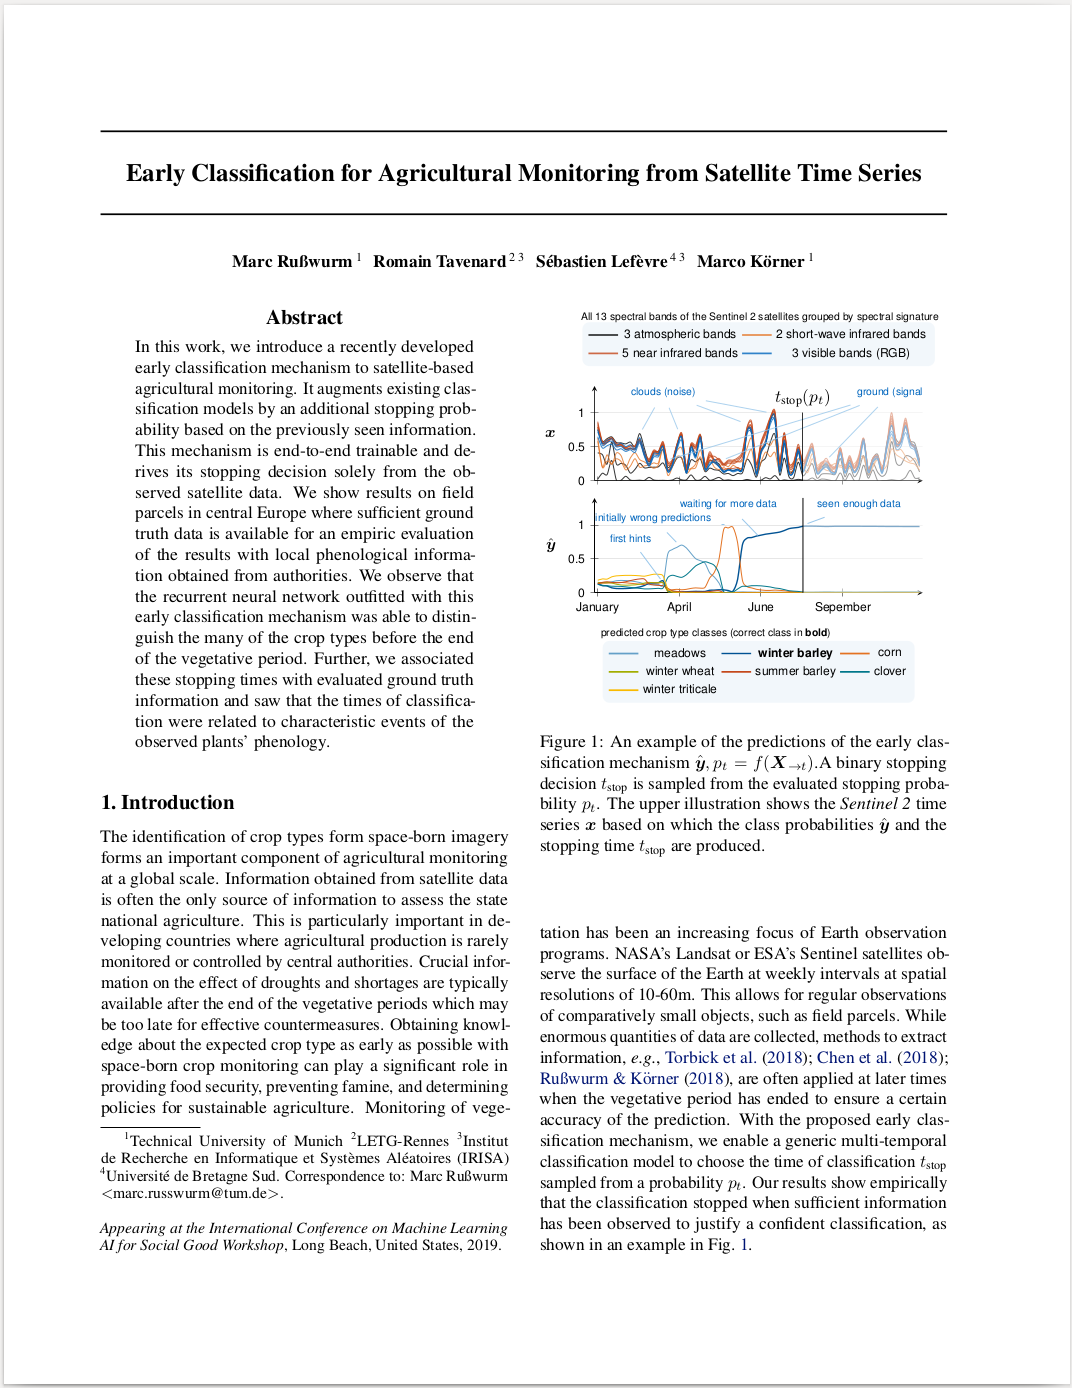
\includegraphics[width=.6\textwidth]{images/AI4SG_Paper}
	
	\end{columns}
\end{frame}

\begin{frame}
	
	\begin{equation}
	P(t;\deltauptot) = \delta_t \cdot \prod_{\tau=0}^{t-1} 1 - \delta_\tau \, .
	\label{eq:pts}
	\end{equation}
	
	\begin{equation}
	\mathcal{L}(\V{x}, \V{y}) = \sum_{t=0}^T P(t;\deltauptot) \mathcal{L}_t(\xuptot, \V{y}) \, .
	\label{eq:ptloss}
	\end{equation}
	
	\begin{equation}
	\mathcal{L}_\text{e}(\xuptot, \V{y} ; \alpha) = \alpha \mathcal{L}_\text{e} (\xuptot, \V{y}) + \left(1-\alpha\right) \mathcal{L}_\text{e}(t)
	\label{eq:lt}
	\end{equation}
	
	\begin{equation}
	\mathcal{L}_\text{e}(t) = \frac{t}{T}
	\label{eq:loss:earliness}
	\end{equation}
	
	\begin{equation}
	\mathcal{L}_t(\xuptot, \V{y} ; \alpha) = \alpha \mathcal{L}_c (\xuptot, \V{y}) - (1 - \alpha)\mathcal{R}_e(t, \ycorrect_t)
	\label{eq:earlyrewardloss}
	\end{equation} 
	
	\begin{equation}
	\mathcal{R}_e(t, \ycorrect_t) = \ycorrect_t \left(1 - \frac{t}{T}\right) \,.
	\label{eq:earlyrewardterm}
	\end{equation}
	
	\begin{equation}
	P^\prime(t;\deltauptot) = P(t;\deltauptot) + \frac{\ptoffset}{T}
	\end{equation}
	
\end{frame}

\begin{frame}
	
		\centering
\tikzstyle{dummy} = [inner sep=0]
\tikzstyle{flow} = [thin, -{Stealth[scale=.5]}]
\tikzstyle{endflow} = [flow, shorten >= 0, shorten <= 0]
\tikzstyle{operator} = [inner sep=0, font=\scriptsize]
\tikzstyle{conn} = [-stealth, shorten >= .2em, inner sep=0]
\tikzstyle{conntime} = [conn, tumgray]
\tikzstyle{lstmcell} = [inner sep=0, fill=tumbluelight!20, rounded corners=1em]


\newcommand{\act}{
	\begin{tikzpicture}[scale=.3]
		\node[circle, draw]{
			\begin{tikzpicture}
			\draw (0,0) to[out=0, in=180] (1,1);
			\end{tikzpicture}
		}
	\end{tikzpicture}	
}



\newcommand{\lstm}{
	\begin{tikzpicture}[inner sep=0, xscale=.5, yscale=.5]
	\coordinate (-input) at (0,1); % top left
	\coordinate (-output) at (0,-2.75); % top left
	\node[inner sep=0](fgate) at (-1.5,0){\fcn};
	\node[inner sep=0](igate) at (-.5,0){\fcn};
	\node[inner sep=0](jgate) at (.5,0){\fcn};
	\node[operator](jmult) at (0,-1.25) {$ \odot $};
	\draw[endflow] (jgate) -- (jmult);
	\draw[endflow] (igate) -- (jmult);
	\node[inner sep=0](ogate) at (1.5,0){\fcn};

	\draw[endflow] (-input) to[out=270,in=90] (ogate.north);
	\draw[endflow] (-input) to[out=270,in=90] (jgate.north);
	\draw[endflow] (-input) to[out=270,in=90] (igate.north); 
	\draw[endflow] (-input) to[out=270,in=90] (fgate.north);

	\node[operator](fmult) at (-1,-1.25) {$ \odot $};
	\draw[endflow] (fgate) -- (fmult); 
	\node[operator](cadd) at (0,-1.75) {$\oplus$};
	\draw[endflow] (jmult) -- (cadd); 
	\draw[endflow] (fmult) -- (cadd);		
	
	\node[operator](outtanh) at (1,-1.25) {$\odot$};
	\draw[endflow] (cadd) -- (outtanh);
	\draw[endflow] (ogate) -- (outtanh);
	
	\node[font=\tiny](c) at (-1,-2){$\V{c}_t$};
	\draw[endflow] (c) -- (fmult);
	\draw[endflow, tumgray] (cadd) -- (c);
	
	\draw (outtanh) to[in=90, out=270] (-output);
	\end{tikzpicture}
}

\newcommand{\legend}{
	\begin{tikzpicture}[yscale=.8, font=\scriptsize]
		\node[label distance=-1em, label={above:fully connected}] at (0,0){$\fcn = \sigma\left(\M{\theta}\V{x}+\V{b}\right)$};
		\node[label={above:hidden state}] at (0,1){$\hidden{6}: \V{a} \in \mathbb{R}^h$};
		\node[label={above:observed state}] at (0,2){$\drawvector{6}: \V{a} \in \mathbb{R}^n$};
%		\node[label={above:mapping}] at (0,3){
%			\begin{tikzpicture}
%				\node(a) at (0,0){$\V{a}_t$};
%				\node(b) at (1.5,0){$\V{a^\prime}_t$};
%				\draw[conn] (a) -- (b);
%			\end{tikzpicture}
%		};
%		\node[label={above:mapping though time}] at (0,4){
%			\begin{tikzpicture}
%			\node(a) at (0,0){$\V{a}_{t-1}$};
%			\node(b) at (1.5,0){$\V{a}_t$};
%			\draw[conntime] (a) -- (b);
%			\end{tikzpicture}
%		};
	\end{tikzpicture}
}

\tikzsetnextfilename{lstmmodel}
\begin{tikzpicture}[node distance=1em and 3em, font=\sffamily]
\node[fill=tumgraylight!20, rounded corners, inner sep=1pt](legend) at (3,-3.5){\legend};

\node[label={left:$\V{x}_t$}](x0){\drawvector{13}};
\node[norm, below= .7em of x0](nx0){\scriptsize LayerNorm};
\node[lstmcell, below=of nx0](l0){\lstm};
\node[below=of l0](l1){\dots};
\node[lstmcell, below=of l1](l2){\lstm};
\node[norm, below=of l2](ny0){\scriptsize LayerNorm};
\node[below=.7em of ny0, label=left:$\V{h}_t$](h){\hidden{16}};


\node[left=2em of l0](ll0){$\text{lstm}^1$};
\node[left=2em of l2](ll2){$\text{lstm}^L$};;
\draw[|-|] (ll0) -- node[midway,left]{$L$ layers} (ll2);

%\node[below left= 2em and 1.3em of h, label={left:$\delta_t$}](d){\drawvector{1}};
%\node[below right= 2em and 1em of h, label={right:$\yhat_t$}](y){\drawvector{6}};
%\draw (h) -- node[fill=white, inner sep=2pt, label={right:}]{\fcn} (y);
%\draw (h) -- node[fill=white, inner sep=2pt, label={left:}]{\fcn} (d);

\draw[conn] (x0) -- (nx0);
\draw[conn] (nx0) -- node[fill=white]{\drawvector{13}} (l0);
\draw[conn] (l0) -- node[fill=white]{\hidden{16}}(l1);
\draw[conn] (l1) -- node[fill=white]{\hidden{16}}(l2);
\draw[conn] (l2) -- node[fill=white]{\hidden{16}}(ny0);
\draw[conn] (ny0) -- (h);

\draw[conntime] (l0)++(-4em,0) -- (l0);
\draw[conntime] (l1)++(-4em,0) -- (l1);
\draw[conntime] (l2)++(-4em,0) -- (l2);

\draw[conntime] (l0) -- ++(4em,0);
\draw[conntime] (l1) -- ++(4em,0);
\draw[conntime] (l2) -- ++(4em,0);

%\node[left=of x0, anchor=east]{\small inputs $x_t$};
%\node[left=of h0, anchor=east]{\small model $f(\xuptot;\theta)$};
%\node[left=of y0, anchor=east]{\small predictions $y_t$};
%
%\node[right=of x0](x1){$x_1$};
%\node[rnn, below=of x1](h1){\small$\theta^{(1)}$};
%\node[rnn, below=of h1](hh1){\small$\theta^{(2)}$};
%\node[below=of hh1](y1){$h_1$};
%\node[below left=1em and -.8em of y1]{$\delta_1$};
%\node[below right=1em and -.8em of y1]{$\hat{y}_1$};
%
%\node[right=of x1](x2){$x_2$};
%\node[rnn, below=of x2](h2){\small$\theta^{(1)}$};
%\node[rnn, below=of h2](hh2){\small$\theta^{(2)}$};
%\node[below=of hh2](y2){$h_2$};
%\node[below left=1em and -.8em of y2]{$\delta_2$};
%\node[below right=1em and -.8em of y2]{$\hat{y}_2$};
%
%\node[right=of x2](x3){};
%\node[right=of h2](h3){};
%\node[right=of hh2](hh3){};
%\node[right=of y2](y3){};
%
%\draw[infer] (h0) -- (h1);
%\draw[infer] (h1) -- (h2);
%\draw[infer] (h3) -- (h3);
%
%\draw[infer] (hh0) -- (hh1);
%\draw[infer] (hh1) -- (hh2);
%\draw[infer] (hh2) -- (hh3);
%
%\foreach \i in {0,...,3}
%{
%	\draw[infer] (x\i) -- (h\i);
%	\draw[infer] (h\i) -- (hh\i);
%	\draw[infer] (hh\i) -- (y\i);
%}

\end{tikzpicture}


	
\end{frame}

\end{document}



